\documentclass{article}

\usepackage{graphicx}
\usepackage{rotating}
\usepackage{amsmath}
\usepackage{amssymb}
\usepackage{fancyhdr}
\usepackage{listings}
\usepackage{xcolor}
\usepackage{color}
\usepackage{amsfonts}
\usepackage{textcomp}
\usepackage{float}
\usepackage{neuralnetwork}
\usepackage[sorting=none]{biblatex}
\usepackage[margin=1in]{geometry}
\usepackage[font={small,it}]{caption}
\usepackage{placeins}
\usepackage{xepersian}

%\DeclareMathOperator*{\btie}{\bowtie}
\addbibresource{bibliography.bib}
\settextfont[Scale=1.2]{B-NAZANIN.TTF}
\setlatintextfont[Scale=1]{Times New Roman}
\renewcommand{\baselinestretch}{1.5}
\pagestyle{fancy}
\fancyhf{}
\rhead{تکلیف اول درس یادگیری عمیق}
\lhead{\thepage}
\rfoot{علیرضا ابره فروش}
\lfoot{9816603}
\renewcommand{\headrulewidth}{1pt}
\renewcommand{\footrulewidth}{1pt}
\newcommand{\Lagr}{\mathcal{L}}
\newcommand{\Mod}[1]{\ (\mathrm{mod}\ #1)}
%%%%%%%%%%
\lstset
{
    language=[latex]tex,
    basicstyle=\ttfamily,
    commentstyle=\color{black},
    columns=fullflexible,
    keepspaces=true,
    upquote=true,
    showstringspaces=false,
    morestring=[s]\\\%,
    stringstyle=\color{black},
}
%%%%%%%%%%
%beginMatlab
\definecolor{mygreen}{RGB}{28,172,0} % color values Red, Green, Blue
\definecolor{mylilas}{RGB}{170,55,241}
%endMatlab
\begin{document}
%beginMatlab
\lstset{language=Matlab,%
    %basicstyle=\color{red},
    breaklines=true,%
    morekeywords={matlab2tikz},
    keywordstyle=\color{blue},%
    morekeywords=[2]{1}, keywordstyle=[2]{\color{black}},
    identifierstyle=\color{black},%
    stringstyle=\color{mylilas},
    commentstyle=\color{mygreen},%
    showstringspaces=false,%without this there will be a symbol in the places where there is a space
    numbers=left,%
    numberstyle={\tiny \color{black}},% size of the numbers
    numbersep=9pt, % this defines how far the numbers are from the text
    emph=[1]{for,end,break},emphstyle=[1]\color{red}, %some words to emphasise
    %emph=[2]{word1,word2}, emphstyle=[2]{style},    
}
%endMatlab
\begin{titlepage}
\begin{center}

\includegraphics[width=0.4\textwidth]{figures/IUT Logo.png}\\
        
\LARGE
\textbf{دانشگاه صنعتی اصفهان}\\
\textbf{دانشکده مهندسی برق و کامپیوتر}\\
        
\vfill
        
\huge
\textbf{عنوان: تکلیف چهارم درس ریزپردازنده}\\
        
\vfill
        
\LARGE
\textbf{نام و نام خانوادگی: علیرضا ابره فروش}\\
\textbf{شماره دانشجویی: 9816603}\\
\textbf{نیم\,سال تحصیلی: پاییز 1400}\\
\textbf{مدرّس: دکتر عارف کریمی افشار}\\
\end{center}
\end{titlepage}


%\tableofcontents
\newpage


%1
\section{}
%$
%m = (00110010)_2 = (50)_{10} \\
%p = 23, q = 19 \\
%n = pq = 23 \times 19 = 437 \\
%z = (p-1)(q-1) = 22 \times 18 = 396 \\
%e = 97 \Rightarrow  e < n,\: (e, z) = 1 \\
%d = 49 \Rightarrow ed \equiv 1 (mod\:z) \\ \\
%c = (m ^ e \equiv 1 (mod \: n)) \Rightarrow c = 335 \\
%m = (c ^ d \equiv 1 (mod \: n)) \Rightarrow m = 50 \\ \\
%K^+ = e = 97 \\
%K^- = d = 49 \\
%$


%2
\section{}
%\lr{Trudy} می‌تواند به سیستم نفوذ کند و محتوای ارسال شده را تغییر دهد. به این صورت که $M$ و $H(M) + S$ را از هم جدا می‌کند. سپس با محاسبه‌ی \lr{hash}ِ پیامِ $M$ و حذف آن از $H(M)+S$ (به شکل $H(M) + S - H(M)$) به \lr{shared secret} دست پیدا می‌کند. سپس پیام مورد نظر خود ($M^{\prime}$) را به همراه $H(M^{\prime})$ و $S$ برای فرد به شکل
%$\left( M^{\prime}, H(M^{\prime}) + S \right)$
%ارسال می‌کند. با اینکه این پروتکل قابلیت نفوذ دارد اما به هر حال نمودار استخراج و \lr{Authentication}ِ پیام به صورت زیر است.
%\begin{figure}[H]
%    \centering
%    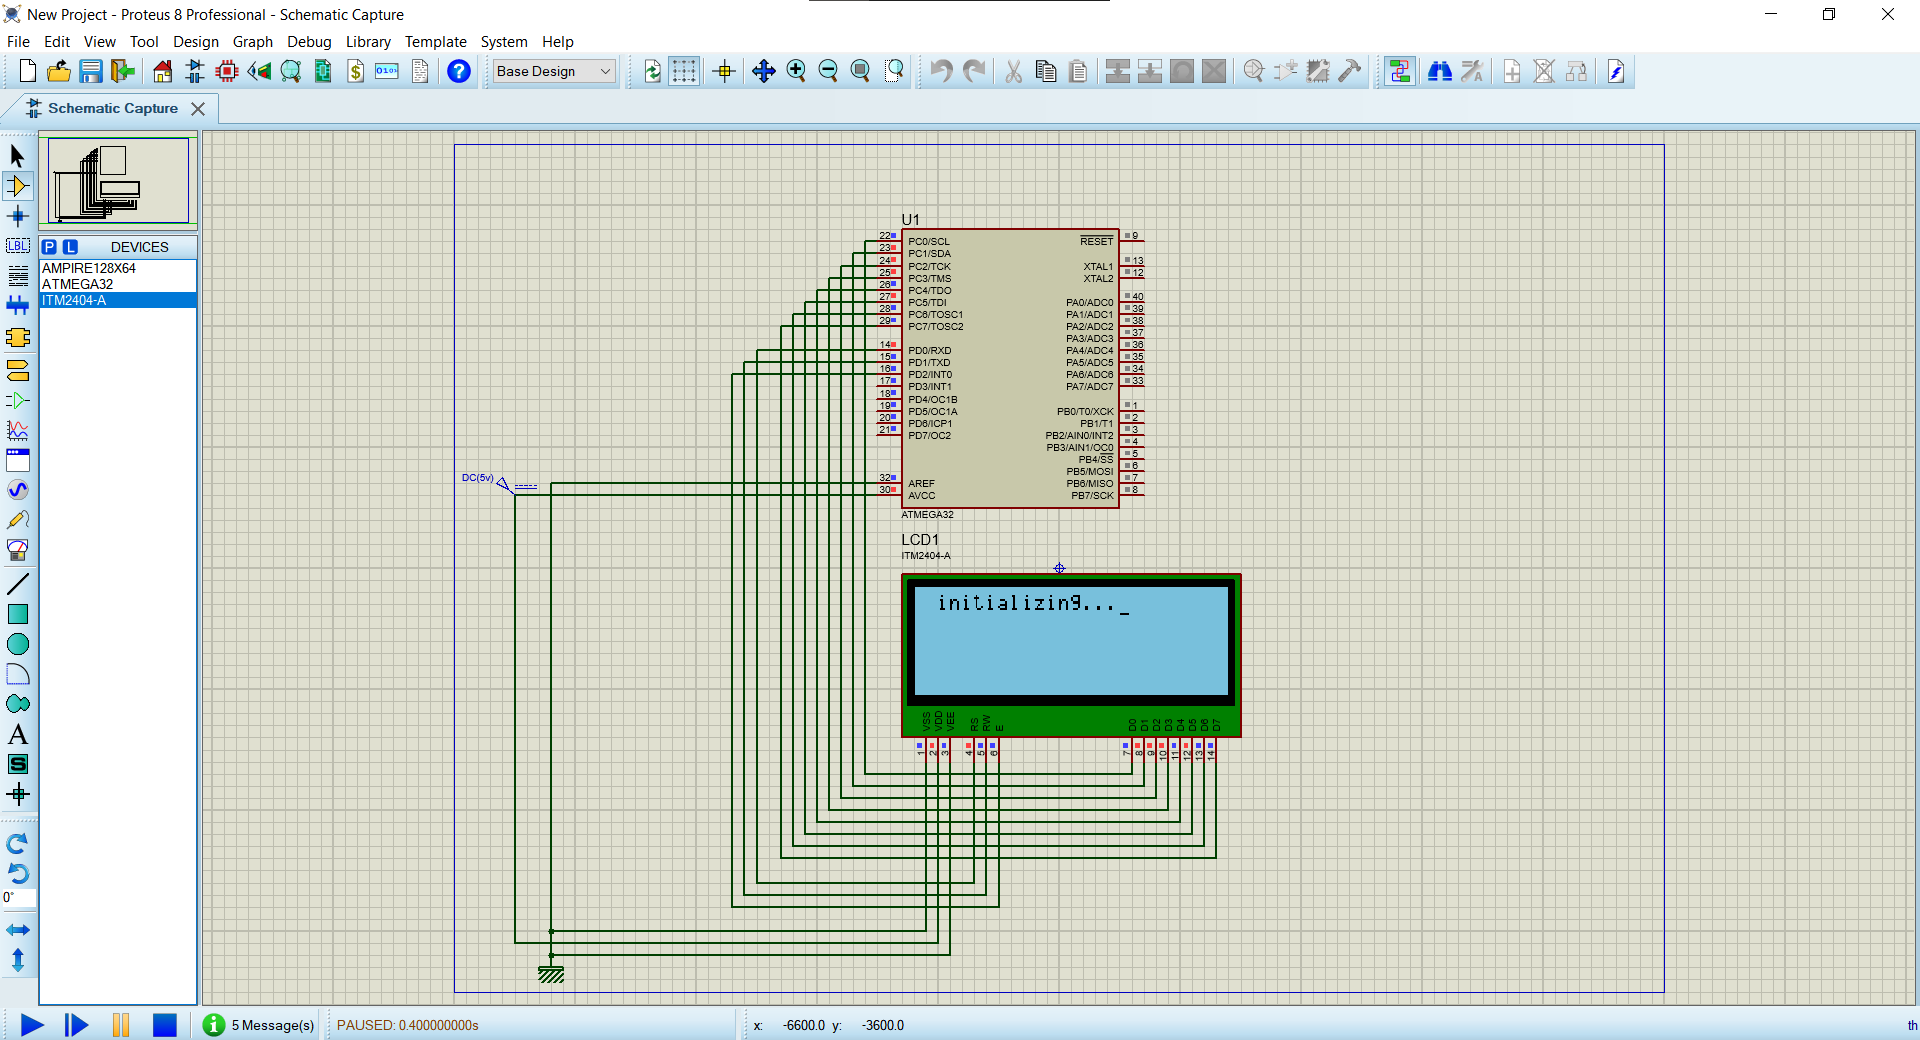
\includegraphics[width=0.50\textwidth]{figures/1.png}
%    \caption
%	{
%نمودار رمزگشایی پیام
%	}
%    \label{fig:fig1}
%\end{figure}


%3
\section{}



%4
\section{}
\begin{latin}
\begin{neuralnetwork}[height=9]
    \newcommand{\x}[2]{$x_#2$}
    \newcommand{\y}[2]{$\hat{y}_#2$}
    \newcommand{\hfirst}[2]{\small $h^{(1)}_#2$}
    \newcommand{\hsecond}[2]{\small $h^{(2)}_#2$}
    \inputlayer[count=4, bias=true, title=Input\\layer, text=\x]
    \hiddenlayer[count=7, bias=true, title=Hidden\\layer, text=\hfirst] \linklayers
    \outputlayer[count=3, title=Output\\layer, text=\y] \linklayers
\end{neuralnetwork}
\end{latin}


%5
\section{}


%6
\section{}


%\begin{enumerate}
%	\item \lr{Bob} لیستی از الگوریتم‌هایی که از آن‌ها پشتیبانی می‌کند را به همراه \lr{nonce} به \lr{Alice} می‌فرستد.
%	\item \lr{Alice} بین لیست الگوریتم‌های پیشنهادی یکی را انتخاب می‌کند و آن را به همراه \lr{certificate} و \lr{nonce} می‌فرستد.
%	\item \lr{Bob} \lr{certificate} را اعتبارسنجی می‌کند، \lr{public key}ِ \lr{Alice} را استخراج می‌کند، \lr{pre\_master\_secret} را تولید می‌کند، با \lr{public key}ِ \lr{Alice} آن را رمز می‌کند و برای \lr{Alice} می‌فرستد.
%	\item \lr{Bob} و \lr{Alice} به طور مستقل رمز و کلیدهای \lr{MAC} را از \lr{pre\_master\_secret} و \lr{nonce}ها محاسبه می‌کنند.
%	\item \lr{Bob} یک \lr{MAC} از همه‌ی پیام‌های \lr{handshake} می‌فرستد.
%	\item \lr{Alice} یک \lr{MAC} از همه‌ی پیام‌های \lr{handshake} می‌فرستد.
%\end{enumerate}




%%%%%%%%%%%%%%%%%%%%%%%%%%%%%%%%%%%
%%%%%%%%%%%%%%%%%%%%%%%%%%%%%%%%%%%
%%%%%%%%%%%%%%%%%%%%%%%%%%%%%%%%%%%



\section*{منابع}
\renewcommand{\section}[2]{}%
\begin{thebibliography}{99} % assumes less than 100 references
%چنانچه مرجع فارسی نیز داشته باشید باید دستور فوق را فعال کنید و مراجع فارسی خود را بعد از این دستور وارد کنید


\begin{LTRitems}

\resetlatinfont

\bibitem{b1} Stošić, Lazar, and Milena Bogdanović. "RC4 stream cipher and possible attacks on WEP." Editorial Preface 3.3 (2012).
\end{LTRitems}

\end{thebibliography}


\end{document}
